\documentclass[10pt,aspectratio=169]{beamer}

% All the boilerplate is in deslides.sty
\usepackage{deslides}

\author{Ji\v{r}\'i Lebl}

\institute[OSU]{%
Oklahoma State University%
%Departemento pri Matematiko de Oklahoma {\^S}tata Universitato%
}

\title{21. Forced oscillations and resonance, \\part 1: Undamped forced motion and resonance\\(Notes on Diffy Qs, 2.6)}

\date{}

\begin{document}

\begin{frame}
\titlepage

%\bigskip

\begin{center}
The textbook: \url{https://www.jirka.org/diffyqs/}
\end{center}
\end{frame}

\begin{frame}
We return to mass on a spring, but now with nonzero forcing function $F(t)$:

\medskip

\hfill\scalebox{0.85}{\subimport*{../figures/}{massfigforce.pdf_t}}\hspace*{\fill}

\medskip
\pause

The equation is
\[
mx'' + cx' + kx = F(t) ,
\]
$m$ is the mass,

$c$ if friction,

$k$ is the spring constant, and

$F(t)$ is an external force acting on the mass.

\medskip
\pause

We consider periodic forces $F(t)$, and the simplest periodic
force is
\[
F(t) = F_0 \cos (\omega t)
\]
\pause
\textbf{Note:} Using Fourier series, all periodic functions can be understood
via this simple case.
\end{frame}

\begin{frame}
We start with undamped ($c=0$) motion:
\[
mx'' + kx = F_0 \cos (\omega t) .
\]
\pause
The complementary solution is
\[
x_c = C_1 \cos (\omega_0 t) + C_2 \sin (\omega_0 t) ,
\qquad
\text{where}
\quad
\omega_0 = \sqrt{\nicefrac{k}{m}} 
\quad = \text{natural (angular) frequency}.
\]
\pause
$\omega_0$ is the frequency
at which the system ``wants to oscillate'' without any force $F$.

\medskip
\pause

First suppose \quad $\omega_0 \not= \omega$.

\medskip
\pause

Using the method of undetermined coefficients we try
\quad
$x_p = A \cos (\omega t)$
\quad and solve for $A$.

\medskip
\pause

(Including $B\sin(\omega t)$ doesn't hurt, you'll see $B=0$).
\pause
We find (exercise)
\[
x_p = \frac{F_0}{m(\omega_0^2 - \omega^2)} \cos (\omega t) .
\]
\pause
\vspace*{-0.2in}

The general solution is

\medskip

\quad $\displaystyle x = C_1 \cos (\omega_0 t) + C_2 \sin (\omega_0 t) +
\frac{F_0}{m(\omega_0^2 - \omega^2)} \cos (\omega t)$
\quad \pause or

\vspace*{-0.05in}

\hspace*{3in}$\displaystyle x = C \cos (\omega_0 t - \gamma) +
\frac{F_0}{m(\omega_0^2 - \omega^2)} \cos (\omega t)$.

\medskip

A superposition of two phase shifted cosine waves at different frequencies.
\end{frame}

\begin{frame}

\textbf{Example:}
Solve \qquad
$0.5 x'' + 8 x = 10 \cos (\pi t), \qquad x(0)=0, \qquad x'(0)=0$.

\medskip
\pause

$\omega = \pi$, ~~ $\omega_0 = \sqrt{\nicefrac{8}{0.5}} = 4$,
~~ $F_0 = 10$, ~~ $m=0.5$.

\medskip
\pause

The general solution is


\quad $x = C_1 \cos (4 t) + C_2 \sin (4 t) +
\dfrac{20}{16 - \pi^2} \cos (\pi t)$.

\pause
\medskip

Solve for $C_1$ and $C_2$ to find

\medskip

\quad $C_1 = \dfrac{-20}{16 - \pi^2}$, \quad $C_2 = 0$, \quad so

\pause
\medskip

\quad $x = 
\dfrac{20}{16 - \pi^2} \bigl( \cos (\pi t)- \cos (4 t) \bigr)$.

\vspace*{-1.7in}
\hfill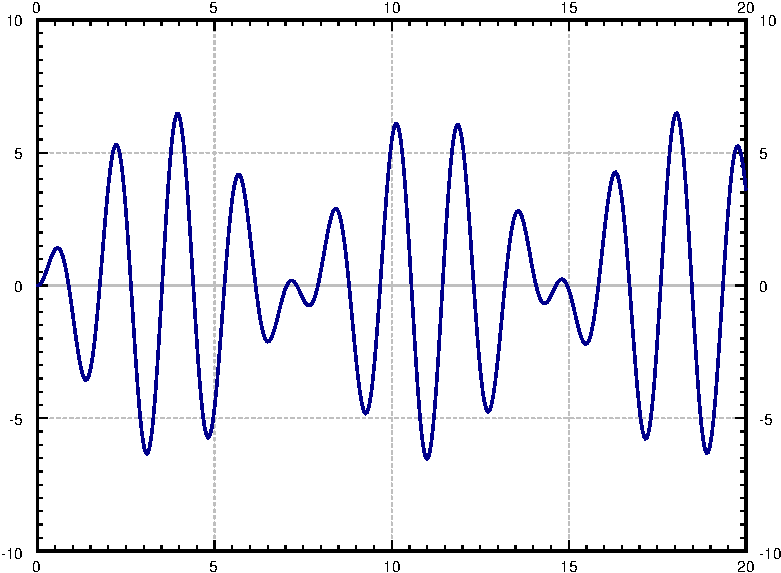
\includegraphics[width=2.7in]{../figures/3-6-beating.pdf}

\vspace*{-0.2in}
\pause

Notice the ``beating'' in the figure.

\medskip
\pause

Using the
identity
\quad
$
2\sin \left( \frac{A-B}{2} \right) \sin \left( \frac{A+B}{2} \right) =
\cos B -\cos A
$,
\quad 
we find
\[
x = 
\frac{20}{16 - \pi^2} \left( 2 \sin \left(\frac{4-\pi}{2} t \right)
\sin \left( \frac{4+\pi}{2} t \right) \right) .
\]
\pause
The solution is a high frequency wave modulated by a low frequency
wave.
\end{frame}


\begin{frame}
What about the case $\omega_0 = \omega$?

\medskip
\pause

From $x_p = \frac{F_0}{m(\omega_0^2 - \omega^2)} \cos (\omega t)$, we suspect
that something ``blows up'' when $\omega$ approaches $\omega_0$.

\medskip
\pause

Undetermined coefficients says we should try
\[
x_p = A t \cos (\omega t) + B t \sin (\omega t)
\qquad \text{(the sine term is needed this time)}.
\]
\pause
Write the equation as
\qquad $x'' + \omega^2 x = \frac{F_0}{m} \cos ( \omega t)$
\qquad and plug in $x_p$ to find
\[
2 B \omega \cos (\omega t) - 2 A \omega \sin (\omega t) = 
\frac{F_0}{m} \cos (\omega t) .
\]
\pause
$A = 0$ and $B = \frac{F_0}{2m\omega}$. \pause  The particular solution is
$\frac{F_0}{2m\omega} \, t \sin (\omega t)$ and the general
\[
x = x_c + x_p = C_1 \cos (\omega t) + C_2 \sin (\omega t)
+ \frac{F_0}{2m\omega} \, t \sin (\omega t) .
\]
Note the $t$ in the $x_p$, so $x_p$ grows without bound as $t \to \infty$.

$x_p$ oscillates between $\frac{F_0 t}{2m\omega}$ and
$\frac{- F_0 t}{2m\omega}$.

$x_c$ only oscillates between
$\pm\sqrt{C_1^2 + C_2^2}$.

\end{frame}

\begin{frame}
For $C_1=C_2=0$, $F_0 = 2$,
$m=1$, $\omega = \pi$,

\medskip

\quad $x = \frac{1}{\pi} t \sin (\pi t)$.

\vspace*{-0.4in}

\hfill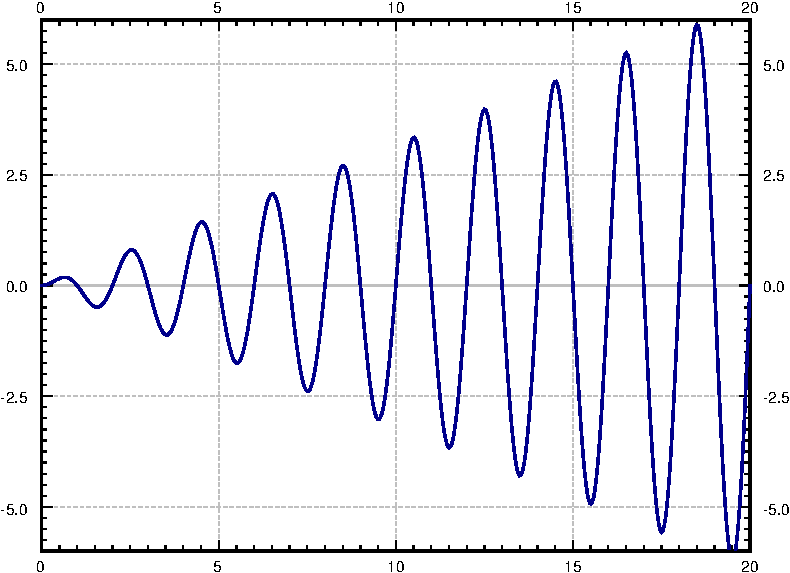
\includegraphics[width=2.7in]{../figures/3-6-resonance.pdf}

\vspace*{-1.55in}

\pause

So when $\omega = \omega_0$, we produce wild

ever growing oscillations.
This behavior

is called \emph{resonance} or
\emph{pure resonance}.

\medskip
\pause

Resonance can be good:

We can create large oscillations

with small force.

\pause

Examples: Swinging a child, quartz watches,

NMR/MRI, \ldots

\medskip
\pause

Resonance can be bad:

Examples: Earthquakes, vibrations in engines, soldiers marching on a bridge,
\ldots

\end{frame}

\end{document}
